\chapter{Preliminaries}
\label{c:preliminaries}
In this section, common techniques of object detection are mentioned. Preprocessing (thresholding, color model transformation,blob detection) and recognition (feature point detection, and matching) are included.

\section{Common Image Processing Techniques}

    \subsection{Color Models}
        In this thesis, two color model were utilized to do the lettering defect detection and LED color \& function inspection.
        There is many different ways to describe colors in image processing.
        \subsubsection{RGB Color Model}
            The color model that most people known was 8 bits RBG color model.
            Which use 8 bits for each channel, could describe 256 X 256 X 256 colors.
            The idea of RGB color space is to separate colors to three primary color that human eyes could sense from light reflected from an object.
            By summing up three different color channel, we could simulate different colors in nature.
            Common used in color LED control and describing the color of a pixel.
            This color model is also the model used to describe raw image captured from camera we used.
        \subsubsection{Gray-scale}
            The color model we used to do lettering defect detection was 8 bit gray-scale color model, this color model could help us in production line to simply parameter setups.
            Also, gray-scale color model performs better then RGB to HSV color model when doing the lettering defect detecting.
            The conversion method from RGB color model to gray-scale color model built in OpenCV is described as below.
            % https://docs.opencv.org/3.1.0/de/d25/imgproc_color_conversions.html
            \begin{center}
            $ Y = 0.299 \times R + 0.587 \times G + 0.114 \times B $
            \end{center}

            Here is an example conversion result.
            \begin{figure}
                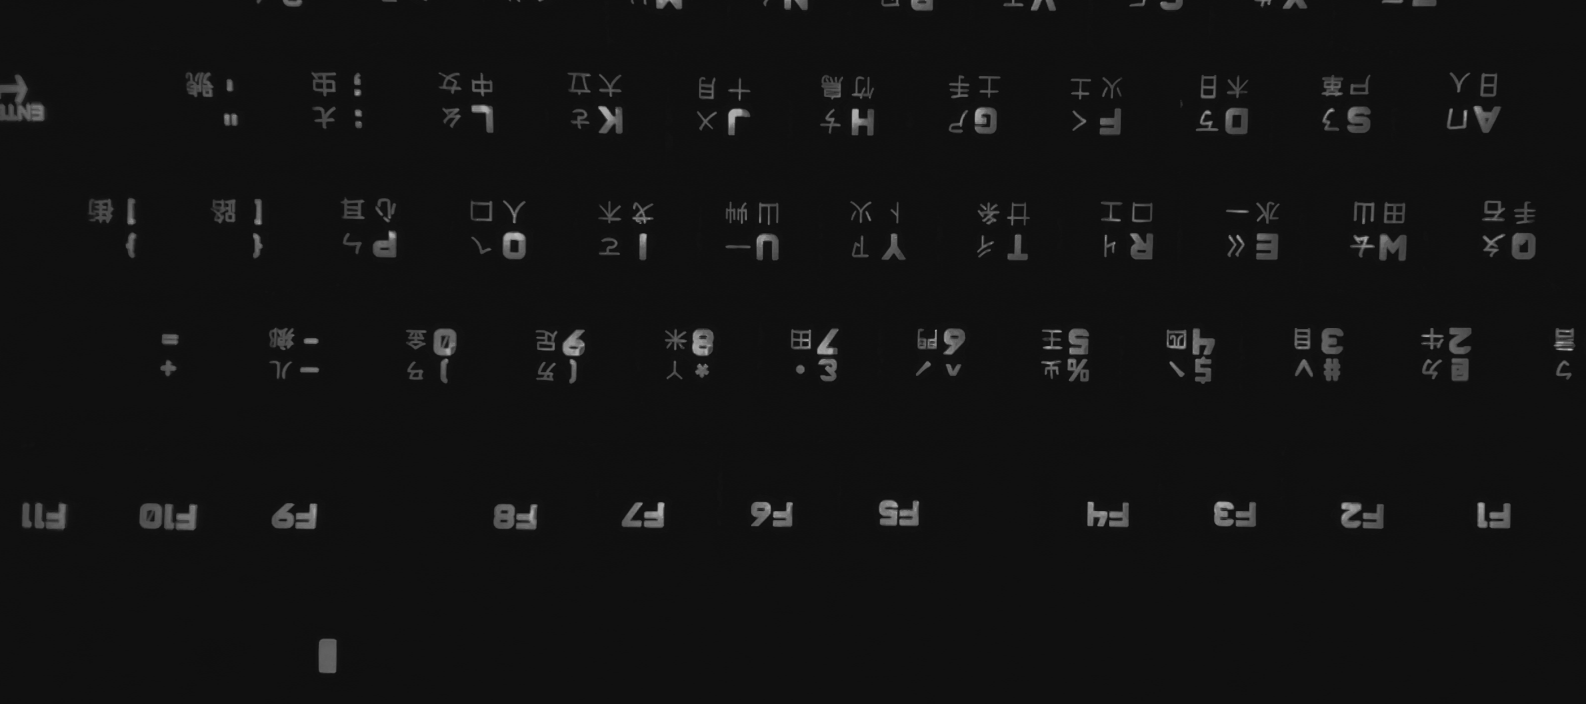
\includegraphics[width=\linewidth]{grayInput.png}
                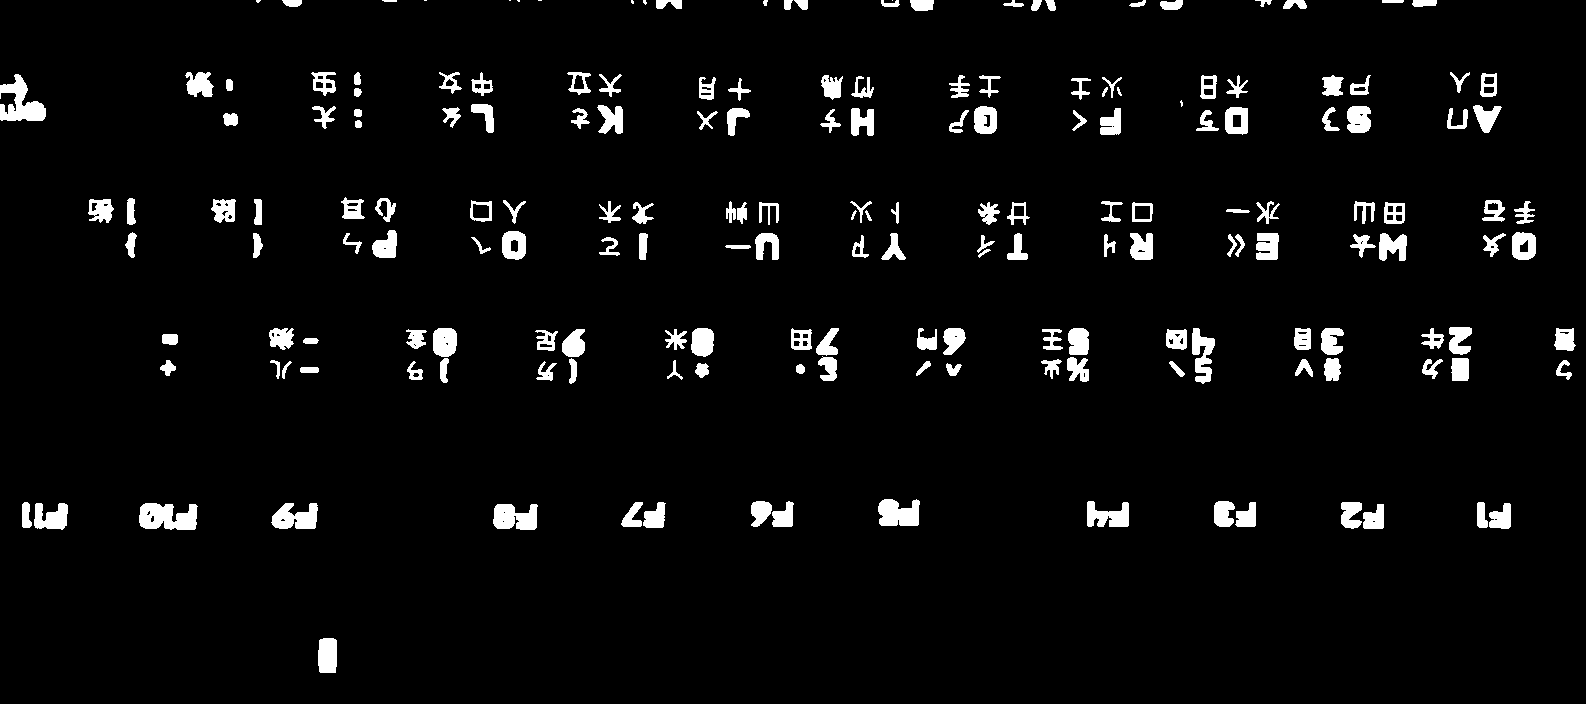
\includegraphics[width=\linewidth]{grayBinaryOutput.png}
                \caption{Grayscale thresholding example.}
                \label{fig:thresholding_Example}
            \end{figure}


        \subsubsection{HSV Color Model}
            The other color model we used was HSV color model, an alternative of RGB color model, this color model describe colors in different way of RGB color model.
            HSV color model use Hue, Saturation and Value to describe different colors.
            This color space could describe different color in a more intuitive way.
            Hue is the parameter represent for the color tone of the pixel. % find formal definition
            Saturation stands for how dense the color is. The more pure pixel color is, the higher value saturation will have.
            Value is used to describe how bright the pixel is. The brighter, the higher.
            The conversion method from RGB color model to HSV color model built in OpenCV is described as below.

            $$
                V = \max(R,G,B)
            $$\\
            $$
                S = 
                \begin{cases}   
                    {{{(V-min(R,G,B))}/{V}}, \enspace\textrm{if}\enspace V \neq 0}\\
                    {0, otherwise}
                \end{cases}
            $$\\
            $$
                H =
                \begin{cases} 
                    {{60(G - B)}/{(V-\min(R,G,B))}, \enspace\textrm{if}\enspace V=R}\\
                    {{120+60(B - R)}/{(V-\min(R,G,B))}, \enspace\textrm{if}\enspace V=G}\\
                    {{240+60(R - G)}/{(V-\min(R,G,B))}, \enspace\textrm{if}\enspace V=B}
                \end{cases}
            $$\\
            $$
                \textrm{If} \enspace H \enspace < \enspace 0 \textrm{, then } H = H + 360. \textrm{ On output } 0 \leq V \leq 1, 0 \leq S \leq 1, 0 \leq H \leq 360
            $$\\
            % \textrm{add HSV filtered example here} 
            \begin{figure}
                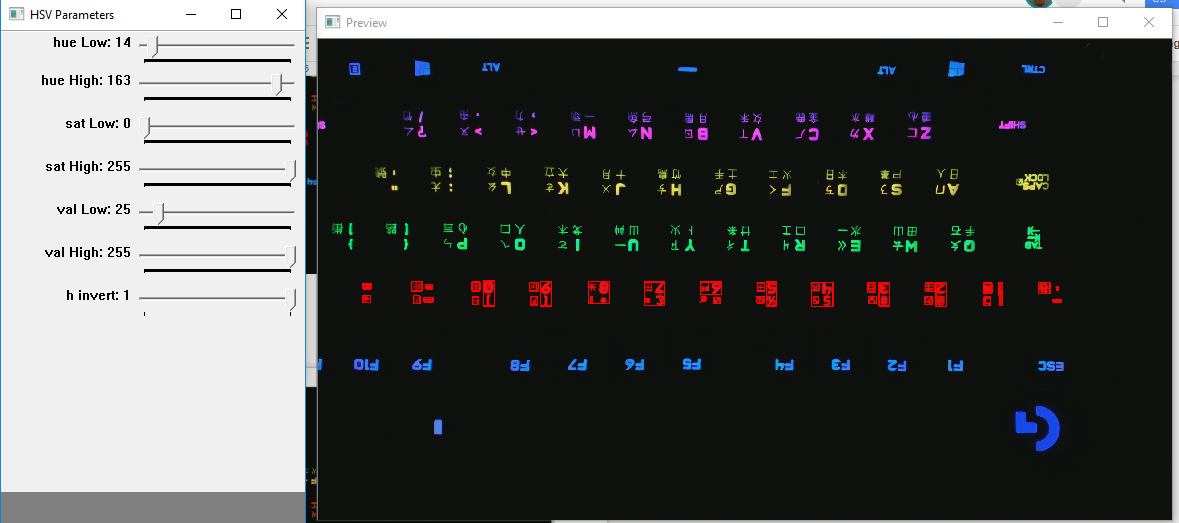
\includegraphics[width=\linewidth]{hsvRed.png}
                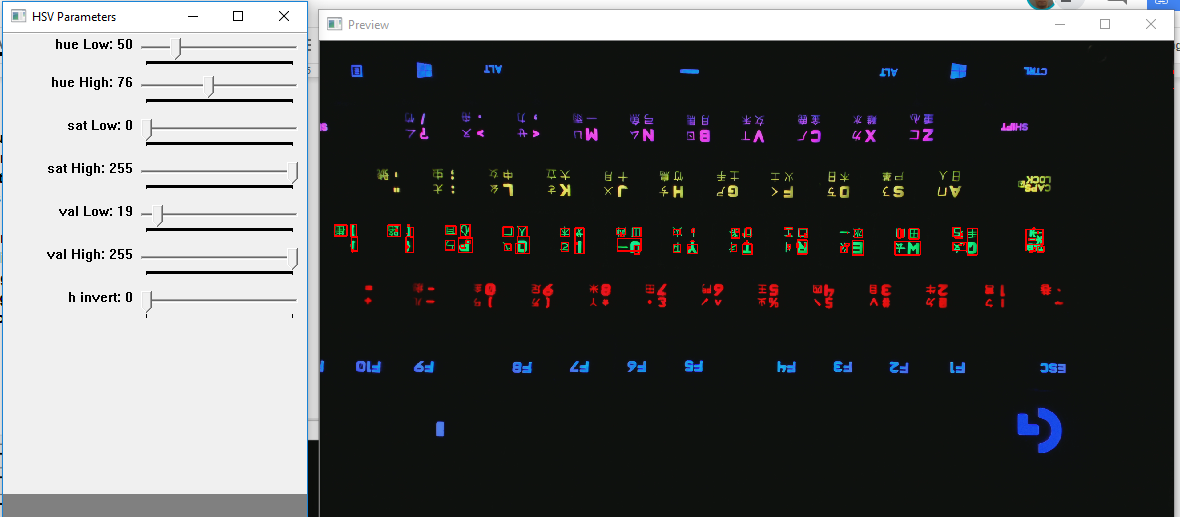
\includegraphics[width=\linewidth]{hsvGreen.png}
                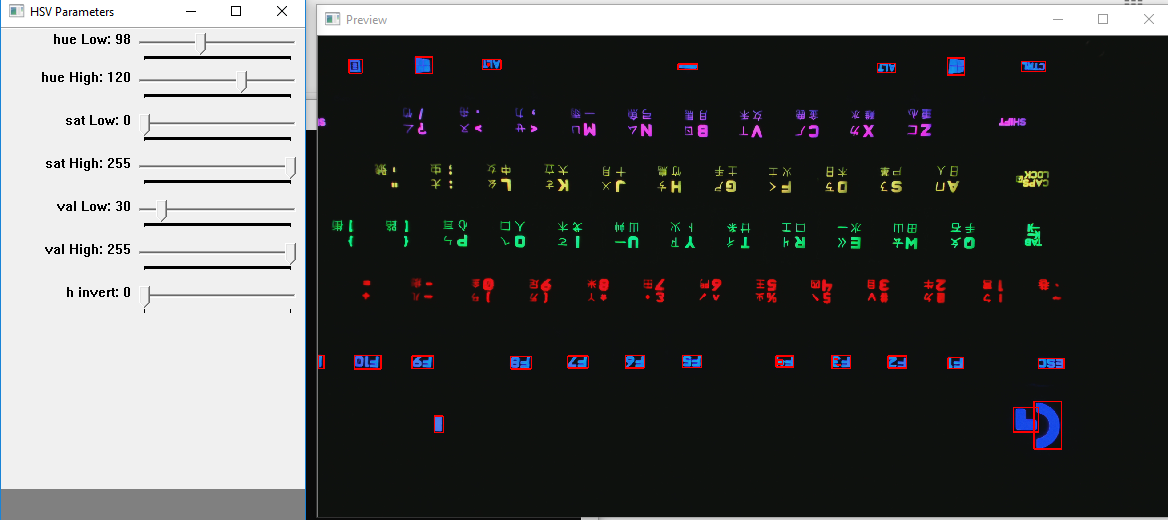
\includegraphics[width=\linewidth]{hsvBlue.png}
                \caption{HSV filtered examples. (RGB color detection)}
                \label{fig:HSV_Example}
            \end{figure}
`'
    \subsection{Thresholding \& Binarization}
        Thresholding with different color model can help us select interested pixels in an efficient way.
        In this thesis, we used this idea to identify where the keyboard buttons are located by doing thresholding to the gray scale image.
        By set a threshold value between 0 \& 255, we can get a binarized image.
        After apply blob or contour detection methods to that  binarized image.
        When thresholding with HSV upper bounds \& lower bounds, we can identify pixels with certain color or brightness.
        By HSV thresholding, we can identify keys with different color lightening.
        Witch is efficient for us to check if the LED back-light is malfunction.
        % add object detection, color detection, shape detection methods.
        $$ \textrm{add example here} $$

    \subsection{Blob Detection}
        % https://www.learnopencv.com/blob-detection-using-opencv-python-c/
        A blob is a group of connected pixels in an image that share some common property (e.g. gray-scale value, HSV value, RGB value, shapes, area, etc).
        The goal of blob detection method is to identify and mark these pixels in the given image.
        In this thesis, after we applied thresholding technique and defect detecting methods to the keyboard image captured from camera and get the corresponding binary image.
        We apply blob detection to that binary image then get the key position, LED color and defect information from it by apply blob detecting with different binary filters.
        $$ \textrm{add example here, grayscale thresholding, HSV filtering.....} $$

    \subsection{Feature Point Detection}
        Feature point detection technique is widely used in object detection or tracking applications.
        Popular methods like SIFT feature points having the current state of the art accuracy, but its slow on execution.
        SURF is an improve based on SIFT feature point. SURF is much faster then SIFT without sacrificing much robustness. But still takes some time when dealing with large sized image. 
        However, by restricting the area of interested with correct parameter setting, SURF feature point could be utilized in our project.
        Other feature point detecting methods like FAST, ORB and FREAK will also be discussed in Chapter 4.

\section{Related Works} 
    % Keywords: Planner object detection, Defect detection, AOI system.
    % this part needs more works to do later.
    % each subsection needs more information.
    This section will introduce where the main concept of each component comes from.
    \subsection{PCB defect detection}
        % https://ieeexplore.ieee.org/stamp/stamp.jsp?tp=&arnumber=5530052
        % defect detecting method referenced from this work.
        Putera et al., \cite{putera2010printed} (2010) proposed a computer vision inspection system implemented with MATLAB.
        The idea of updated defect detection method for keyboard lettering is from this work.

    \subsection{Computer-Vision-Based Fabric Defect Detection}
        % https://ieeexplore.ieee.org/stamp/stamp.jsp?tp=&arnumber=4418522
        % where multiple camera idea from
        Kumar et al.,(2008)\cite{kumar2008computer} gives a design of CV based inspection platform for fabric defect detecting.
        We applied the idea connect multiple camera to one host machine in this thesis.

    \subsection{Image Alignment}
        % https://www.learnopencv.com/image-alignment-feature-based-using-opencv-c-python/
        % https://www.learnopencv.com/image-alignment-ecc-in-opencv-c-python/
        On the website owned by Satya Mallick, he showed two different way to do the image alignment.
        One is by enhanced correlation coefficient (ECC) \cite{ECC_Alignment}, the other is based on feature point matching \cite{featureBasedAlignment}.

\section{Previous Solution}
    % give more detailed introduction on previous solution.
    Previous solution applied SURF feature point on every ROI that represented a key, and we found that feature point based method have accuracy issue on small target searching at production line.
    Also, the lettering defect detecting method is not sensitive enough to deal with small defect.
    In this thesis, we'll focus on how to correct these problems.